\documentclass{article}
\usepackage[utf8]{inputenc}
\usepackage{amsmath}
\usepackage{amssymb}
\usepackage{graphicx}
\usepackage{algorithm}
\usepackage{algorithmic}
\usepackage{hyperref}
\usepackage[a4paper, total={6in, 8in}]{geometry}

\title{Problema do Trabalho Balanceado}
\author{Gustavo Delazeri}
\date{12 de Agosto de 2020}

\begin{document}

\maketitle

\section{Introdução}
\quad O objetivo deste trabalho é implementar, calibrar e testar um algoritmo genético para resolver o problema do Trabalho Balanceado. 
O problema do Trabalho Balanceado é assim definido: dados um conjunto de $n$ tarefas que precisam ser executadas em sequência, um conjunto de $m$ operadores e uma matriz $p$, onde $p_{ij}$ representa o tempo necessário para o trabalhador $j$ executar a tarefa $i$, encontre  uma partição das $n$ tarefas em $m$ intervalos $[b_{k}, e_{k}] \, k \in [m] $ e uma permutação dos
operadores $\pi$ de forma que  $T =  max_{j \in [m]} T_{j}$ é minimizado, sendo que $T_{j} = \sum_{t \in [b_{t}, e_{t}]}{} p_{t\pi_{j}} $. Em outras palavras, encontre uma atribuição de tarefas a operadores de tal modo que operadores executem tarefas sequenciais e o tempo gasto pelo operador que gasta mais tempo trabalhando é minimizado. 
\section{Formulação do Problema como Programa Inteiro}
\textbf{Variáveis:} 
\begin{itemize}
  \item $x_{ij} \in \{0, 1\}, \quad \forall i,j  \, \mid  \, i \in [n] \land j \in [m]$, onde
  	$$x_{ij} = 
	\begin{cases}
	1,  \quad  \text{Caso tarefa i e executada pelo operador j } \\
	0,  \quad  \text{Caso contrario}
	\end{cases}
	$$
  \item $w_{ijk} \in \{0, 1\}, \quad \forall i,j,k  \, \mid \,  i,j \in [n]  \land k \in [m] \land i \neq j$, onde
  	$$w_{ijk} = 
	\begin{cases}
	1,  \quad  \text{Caso } \,  x_{ik} \land x_{jk} \, \text{é verdade }\\
	0,  \quad  \text{Caso contrario}
	\end{cases}
	$$
	
  \item $y \in \mathbb{R}$, onde
  	$$y = \text{max}\Bigg(\sum_{i \in [n] }^{} p_{ij} \cdot x_{ij},   \forall j \in [m] \Bigg)	$$
\end{itemize}
\textbf{Função Objetivo:} 
	$$\text{Min.} \quad y$$
\textbf{Restrições:} 

\begin{equation}
 	\sum_{j \in [m] }^{} x_{ij} = 1,   \quad \forall i \in [n] 
\end{equation}

\begin{equation}
 	\sum_{i \in [n] }^{} x_{ij}  \geq 1,  \quad  \forall j \in [m] 
\end{equation}

\begin{equation}
 	w_{ijk} \leq (x_{ik} + x_{jk})/2, \quad \forall i,j,k \, \mid \, i,j \in [n]  \land k \in [m] \land i < j
\end{equation}

\begin{equation}
 	w_{ijk} \geq x_{ik} + x_{jk} - 1,  \quad \forall i,j,k \, \mid \, i,j \in [n]  \land k \in [m] \land i < j
\end{equation}

\begin{equation}
 	w_{ijk} \leq x_{j-1k},  \quad \forall i,j,k \, \mid \, i,j \in [n]  \land k \in [m] \land i < j
\end{equation}

\begin{equation}
 	y \geq \sum_{i \in [n] }^{} p_{ij} \cdot x_{ij},   \quad \forall j \in [m]
\end{equation}

A restrição (1) garante que toda tarefa é executada por exatamente 1 operador. A restrição (2) garante que todo operador executa pelo menos uma tarefa. Restrições (3) e (4) formam uma conjunção: se as tarefas i e j são executadas pelo mesmo operador $k$, então $w_{ijk}$ é verdade. A restrição (5) garante que operadores só executam tarefas sequenciais. Por exemplo, um operador não pode executar as tarefas 1,2 e 4. A restrição (6) define um limite inferior para a variável $y$, a qual representa o tempo gasto pelo operador que trabalha por mais tempo.

\section{O Algoritmo Genético}
\subsection{Parâmetros}
\quad A tabela abaixo apresenta os parâmetros do algoritmo e a notação adotada.
\begin{table}[ht]
\centering
\begin{tabular}{c|l}
\hline
$\mu$ & Quantidade de indivíduos na população inicial \\ \hline
$\lambda$ & Quantidade de novos individuos gerados \\ \hline
$k$ & Número de participantes de um torneio aleatório \\ \hline
$\phi$ & Probabilidade de um indivíduo sofrer mutação \\ \hline
$\omega$ & Número máximo de gerações consecutivas que não alteram a melhor solução \\ \hline
\end{tabular}
\end{table}\subsection{Codificação de uma Solução}
\quad Uma solução para uma instância de $n$ tarefas e $m$ operadores é representada por um vetor $v$ de inteiros não negativos de tamanho $n$. Se $v_{i} = j$ então o operador $j$ executa a tarefa $i$. A figura abaixo ilustra a codificação de uma solução de uma instância com 6 tarefas e 4 operadores.
\begin{figure}[tph!]
\centering
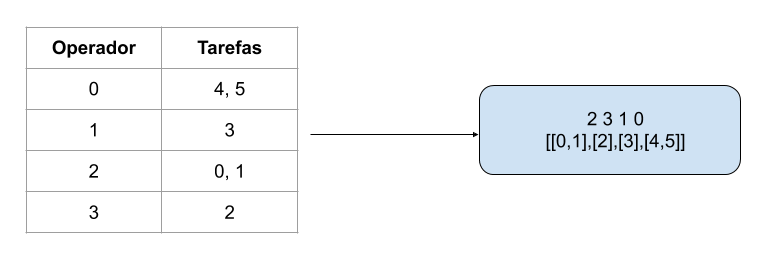
\includegraphics[scale=0.35]{figure1}
\end{figure}


\newpage
\subsection{População Inicial}
\quad A população inicial é gerada aleatoriamente. Primeiro criam-se $\mu$ permutações e depois $\mu$ partições. Por último, associa-se a cada permutação uma partição, também de forma aleatória. A tabela abaixo ilustra o processo considerando uma instância de 8 tarefas e 4 operadores.
\begin{table}[!htp]
\centering
\begin{tabular}{ccc}
\hline
\textbf{Permutação} & \textbf{Partição} & \textbf{Indivíduo Gerado} \\ \hline
(0 3 2 1) & 0 0 1 1 2 2 3 3 & 0 0 3 3 2 2 1 1 \\ \hline
(2 3 0 1) & 0 1 1 1 2 3 3 3 & 2 3 3 3 0 1 1 1 \\ \hline
(3 1 0 2) & 0 0 0 0 0 1 2 3 & 3 1 0 0 0 0 0 2 \\ \hline
(1 2 3 0) & 0 1 2 2 2 3 3 3 & 1 2 2 2 3 3 3 0 \\ \hline
\end{tabular}
\end{table}

\subsection{Seleção de Indivíduos para Crossover}
\quad A seleção de indivíduos para crossover implica na realização de $\lambda$ $k$-torneios aleatórios. Um $k$-torneio aleatório consiste em selecionar $k$ indivíduos da população de forma aleatória e escolher o melhor desses $k$ indivíduos.
 
\subsection{Crossover}
\quad O processo de crossover consiste em criar duas novas soluções usando a partição/permutação de um pai com a partição/permutação do outro. A figura abaixo ilustra o processo. O indivíduo 3 herda a permutação do indivíduo 2 (1 0 2 3)  e a partição do indivíduo 1 (um 0, três 1's, três 2's e três 3's). Já o indivíduo 4 herda a permutação do indivíduo 1 (3 1 2 0) e a partição do indivíduo 2 (dois 0's, três 1's , três 2's e dois 3's).
\begin{figure}[tph!]
\centering
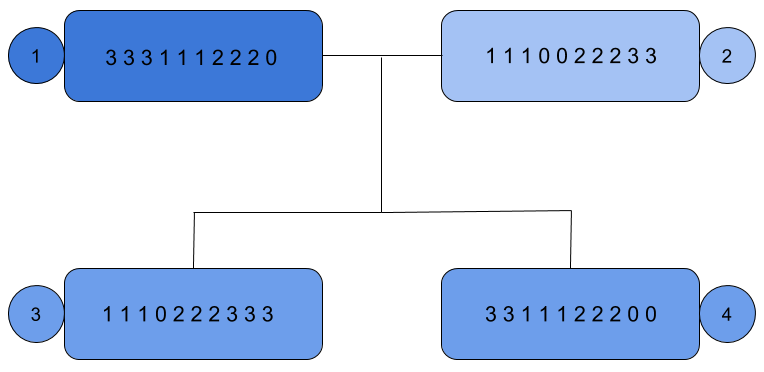
\includegraphics[scale=0.35]{figure2}
\end{figure}

\subsection{Mutação}
\quad O processo de mutação tem duas etapas. A primeira consiste em gerar um número aleatório $k\in \{1, 2, 3,...,10\}$ e aplicar $k$ pequenas perturbações na permutação da solução. A segunda etapa consiste em escolher dois operadores $w_{1}$ e $w_{2}$ aleatoriamente, sendo que $w_{1}$ terá seu intervalo $l$ unidades maior e $w_{2}$ terá seu intervalo $l$ unidades menor. O valor de $l$ é um número aleatório maior ou igual a zero e menor ou igual à metade da magnitude do intervalo de $w_{2}$. A figura abaixo ilustra o processo para $k=2$, $w_{1} = 1$, $w_{2} = 3$ e $l=1$.
\begin{figure}[tph!]
\centering
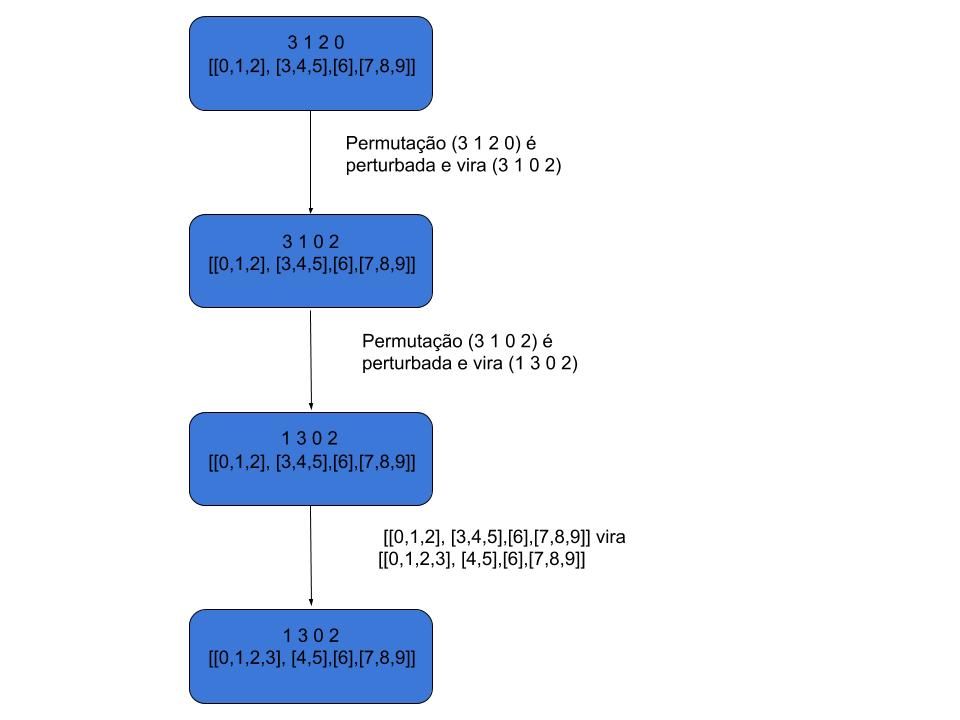
\includegraphics[scale=0.35]{figure3}
\end{figure}

\subsection{Seleção da Nova População}
\quad A seleção da nova população depende do parâmetro $\lambda$ . Se $\lambda$ novos indivíduos foram criados via crossover, então os $\lambda$ piores indivíduos  entre todos os indivíduos (geração atual e nova geração) são eliminados da população.


\subsection{Critério de Parada}
\quad A execução do algoritmo para e retorna uma solução se $\omega$ gerações consecutivas foram geradas e o valor da função objetivo não diminuiu.

\subsection{Pseudocódigo}
\begin{algorithm}[H]
\caption{Algoritmo Genético}
\begin{algorithmic}

\STATE $populacao \leftarrow populacaoInicial(\mu)$
\STATE $M \leftarrow melhorIndividuo(populacao)$
\STATE $geracoesSemMelhora \leftarrow 0$
\WHILE{$geracoesSemMelhora < \omega$}
\FOR{$i \in [\frac{\lambda}{2}] $}
\STATE $pai \leftarrow torneioAleatorio(populacao, k)$
\STATE $mae \leftarrow torneioAleatorio(populacao, k)$
\STATE $filho1, filho2 \leftarrow crossover(pai, mae)$
\IF{$random\lbrack0,1) < \phi$}
\STATE $filho1 \leftarrow mutacao(filho1)$
\ENDIF
\IF{$random\lbrack0,1) < \phi$}
\STATE $filho2 \leftarrow mutacao(filho2)$
\ENDIF
\STATE $populacao \leftarrow populacao \cup \{filho1, filho2\}$
\ENDFOR
\STATE $populacao \leftarrow removePioresIndividuos(populacao, \lambda) $
\STATE $N \leftarrow melhorIndividuo(populacao)$
\IF{$N$ é pior ou igual a $M$}
\STATE $geracoesSemMelhora \leftarrow geracoesSemMelhora + 1$
\ELSE
\STATE $M \leftarrow N$
\STATE $geracoesSemMelhora \leftarrow 0$
\ENDIF
\ENDWHILE
\RETURN $M$
\end{algorithmic}
\end{algorithm}


\subsection{Implementação}

\subsubsection{Plataforma e Linguagem de Programação}
\quad O algoritmo genético foi implementado em Python e usa somente bibliotecas padrão da linguagem.  A plataforma utilizada possui sistema operacional macOS Catalina, versão 10.15.6, com um
processador Intel(R) Core(TM) i5, com 2 núcleos físicos de 2.3GHz, com cache L2 de 256KB (em cada núcleo) e 8GB de memória.

\subsubsection{Estruturas de Dados}
\quad A representação de um indivíduo (cromossomo) é feita utilizando uma lista de tamanho $n$. Visando facilitar as operações de mutação e crossover, a permutação de operadores e o tamanho do intervalo de cada operador são armazenados durante a execução usando listas de tamannho $m$ e $n$, respectivamente.

\subsubsection{Cálculo do fitness de um indivíduo}
\quad Para calcular o fitness de um indivíduo é necessário percorrer a lista que representa o cromossomo e armazenar o tempo gasto por cada operador em uma lista de tamanho $m$. Retorna-se, então, o maior valor da lista de tamanho $m$.

\section{Resultados Numéricos}
\quad Os testes realizados dividem-se em duas categorias: teste de parâmetros e teste das instâncias. Os testes de parâmetros servem para calibrar o algoritmo genético. Os testes das instâncias servem para  comparar o algoritmo genético com a resolução via programação inteira mista usando um solver. Todas as instâncias usadas nos testes podem ser encontradas em \url{http://www.inf.ufrgs.br/~mrpritt/oc/trsp.zip}

\subsection{Teste de Parâmetros}
\quad Para os testes de parâmetros  definiu-se uma configuração base arbitrária, a partir da qual cada parâmetro apresentado na tabela da seção 3.1 é variado individualmente. A configuração base é mostrada abaixo. Para cada variação de parâmetro, o valor da solução associada é a média aritmética das soluções encontradas para as instâncias $tba1$, $tba1$ e $tba3$. O valor da solução de cada instância é a média aritmética de 5 execuções.
\begin{table}[!htp]
\centering
\begin{tabular}{ccccc}
\hline
$\mu$ & $\lambda$ & $k$  & $\phi$ & $\omega$ \\ \hline
500 & 100 & 3 & 0.5 & 500 \\ \hline
\end{tabular}
\end{table}

\subsubsection{$\mu$ - Tamanho da população inicial}
\quad O valor de $\mu$ foi variado de 100 a 1500 com incrementos de 100. A figura abaixo mostra os resultados.
\begin{figure}[H]
\centering
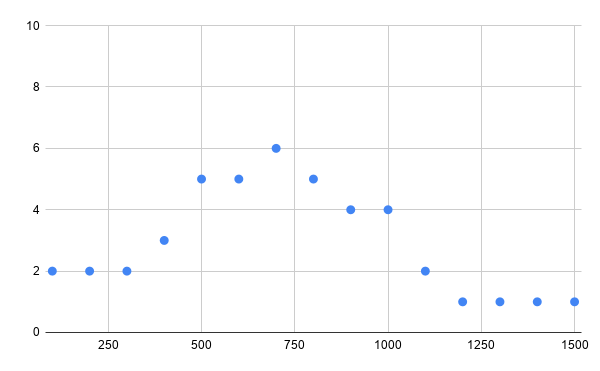
\includegraphics[scale=0.35]{placeholder}
\end{figure}
\quad tiam sit amet lectus nec magna aliquet convallis. Curabitur sed lobortis nulla, sed imperdiet libero. Morbi rhoncus eros nec nisi auctor egestas. Quisque ut nisl dictum lectus mollis tristique rutrum eget arcu. Sed sit amet blandit sapien, eget pulvinar enim. Praesent scelerisque quam a leo pellentesque, a congue arcu luctus. Integer augue urna, vestibulum et nulla vel, lacinia volutpat neque.

\subsubsection{$\lambda$ - Tamanho da prole}
\quad O valor de $\lambda$ foi variado de 10 a 200 com incrementos de 10. A figura abaixo mostra os resultados.
\begin{figure}[H]
\centering
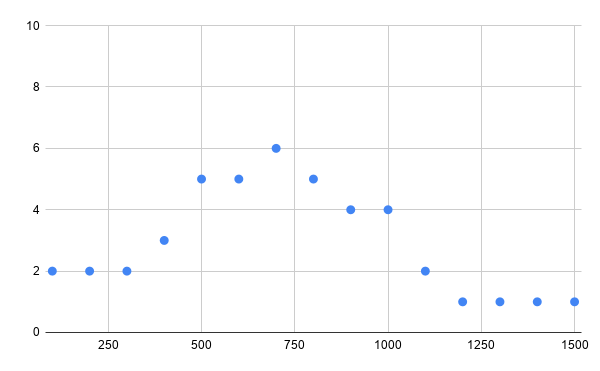
\includegraphics[scale=0.35]{placeholder}
\end{figure}
\quad tiam sit amet lectus nec magna aliquet convallis. Curabitur sed lobortis nulla, sed imperdiet libero. Morbi rhoncus eros nec nisi auctor egestas. Quisque ut nisl dictum lectus mollis tristique rutrum eget arcu. Sed sit amet blandit sapien, eget pulvinar enim. Praesent scelerisque quam a leo pellentesque, a congue arcu luctus. Integer augue urna, vestibulum et nulla vel, lacinia volutpat neque.

\subsubsection{$k$ - Número de participantes de um torneio aleatório}
\quad O valor de $k$ foi variado de 3 a 20 com incrementos unitários. A figura abaixo mostra os resultados.
\begin{figure}[H]
\centering
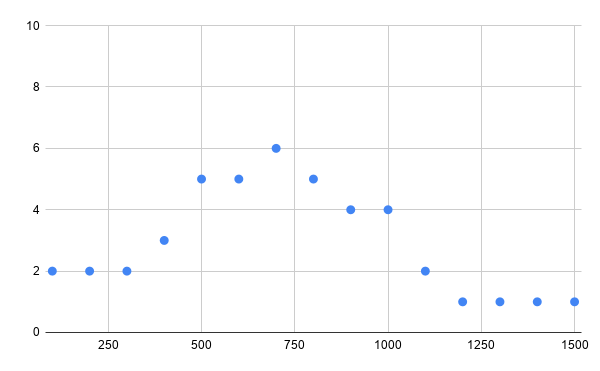
\includegraphics[scale=0.35]{placeholder}
\end{figure}
\quad tiam sit amet lectus nec magna aliquet convallis. Curabitur sed lobortis nulla, sed imperdiet libero. Morbi rhoncus eros nec nisi auctor egestas. Quisque ut nisl dictum lectus mollis tristique rutrum eget arcu. Sed sit amet blandit sapien, eget pulvinar enim. Praesent scelerisque quam a leo pellentesque, a congue arcu luctus. Integer augue urna, vestibulum et nulla vel, lacinia volutpat neque.

\subsubsection{$\phi$ - Probabilidade de um indivíduo sofrer mutação}
\quad O valor de $\phi$ foi variado de 0.1 a 1 com incrementos de 0.1. A figura abaixo mostra os resultados.
\begin{figure}[H]
\centering
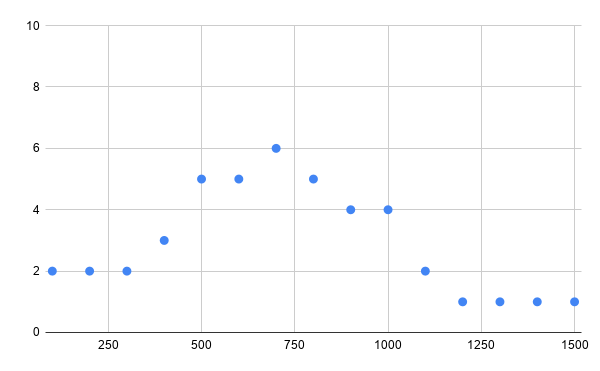
\includegraphics[scale=0.35]{placeholder}
\end{figure}
\quad tiam sit amet lectus nec magna aliquet convallis. Curabitur sed lobortis nulla, sed imperdiet libero. Morbi rhoncus eros nec nisi auctor egestas. Quisque ut nisl dictum lectus mollis tristique rutrum eget arcu. Sed sit amet blandit sapien, eget pulvinar enim. Praesent scelerisque quam a leo pellentesque, a congue arcu luctus. Integer augue urna, vestibulum et nulla vel, lacinia volutpat neque.

\subsubsection{$\omega$ - Número máximo de gerações consecutivas que não alteram a melhor solução}
\quad O valor de $\omega$ foi variado de 100 a 1000 com incrementos de 100. A figura abaixo mostra os resultados.
\begin{figure}[H]
\centering
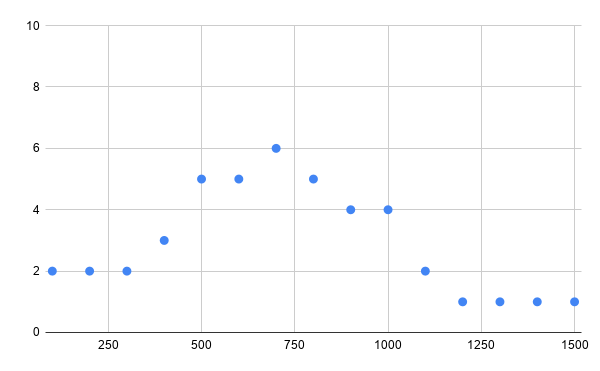
\includegraphics[scale=0.35]{placeholder}
\end{figure}
\quad tiam sit amet lectus nec magna aliquet convallis. Curabitur sed lobortis nulla, sed imperdiet libero. Morbi rhoncus eros nec nisi auctor egestas. Quisque ut nisl dictum lectus mollis tristique rutrum eget arcu. Sed sit amet blandit sapien, eget pulvinar enim. Praesent scelerisque quam a leo pellentesque, a congue arcu luctus. Integer augue urna, vestibulum et nulla vel, lacinia volutpat neque.


\subsection{Teste de instâncias}
\quad O algoritmo genético e o solver foram executados em 10 instâncias diferentes. A tabela abaixo resume o conjunto de instâncias.


\subsubsection{Algoritmo Genético}
\quad O algoritmo genético foi calibrado usando os melhores resultados de cada parâmetro nos testes apresentados na seção 4.1. A tabela e a figura abaixo apresentam a configuração final de parâmetros do algoritmo genético e os resultados obtidos, respectivamente.
\begin{table}[!htp]
\centering
\begin{tabular}{ccccc}
\hline
$\mu$ & $\lambda$ & $k$  & $\phi$ & $\omega$ \\ \hline
1500 & 100 & 3 & 0.5 & 1000 \\ \hline
\end{tabular}
\end{table}

\begin{figure}[H]
\centering
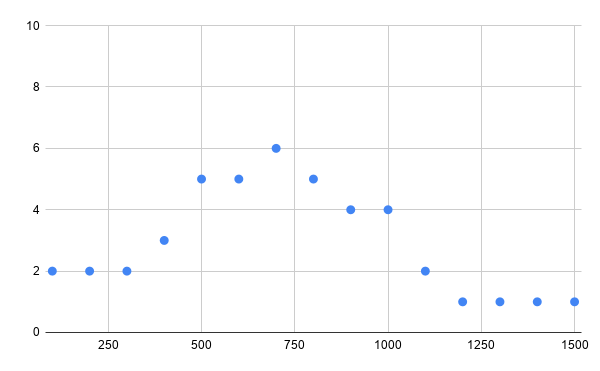
\includegraphics[scale=0.35]{placeholder}
\end{figure}


\subsubsection{Execução com o solver}
\quad O solver usado na resolução das instâncias foi o CPLEX, junto com um tempo limite de 1800 segundos  para o retorno de uma solução. A figura abaixo apresenta os resultados
\begin{figure}[H]
\centering
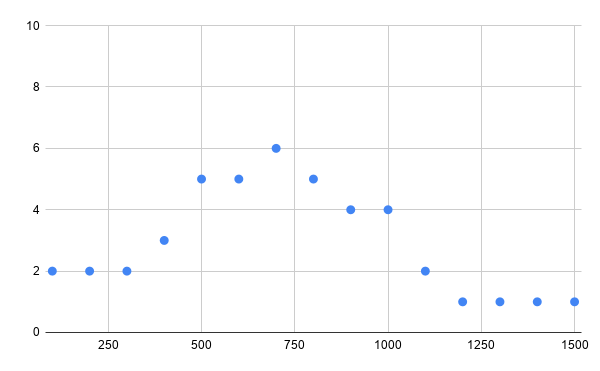
\includegraphics[scale=0.35]{placeholder}
\end{figure}


\section{Conclusão}

\end{document}

